\section{Method}\label{sec:yourmethod}
In this section, start with an overview of the FW instances we examine, and the infrastructure we work with. Then, we briefly describe our process of writing baseline implementations, and then implementing various optimizations.

This work is focused on three particular semi-rings, each giving rise to its own instance of the Floyd-Warshall algorithm, targeted at solving its own problem.
\begin{itemize}
\item The semi-ring \(\langle \mathbb{R}^{\infty},\min,+\rangle\) corresponds to the all-pairs \emph{shortest-path problem} (APSP). It computes the length of the shortest path between every pair of vertices in a graph.
\item The semi-ring \(\langle \mathbb{R}^{\infty},\max,\min\rangle\) corresponds to the all-pairs \emph{widest-path problem} (MM). It maximizes the smallest weight, a path between every pair of vertices has.
\item The semi-ring \(\langle \{0, 1\},\lor,\land\rangle\) corresponds to the \emph{transitive closure} (TC). It checks for every pair of vertices, if one is reachable from the other.
\end{itemize}

For each of these three semi-rings, we start by writing simple reference implementations in \emph{Python} and \emph{Go}. These are not used for benchmarking purposes, but to ensure our later implementations are correct and produce the same results.

Next, we write and benchmark a naive baseline implementation for each semi-ring. Due to the algorithm's simplicity, many of the more standard optimization techniques like strength reduction or function inlining are not possible. For this reason, we optimize FW by implementing the previously introduced \texttt{FWI} and \texttt{FWT} algorithms for the three listed FW instances. Additionally, we implement vectorized versions of the resulting 6 implementations.

Lastly, we implement and evaluate an autotuner, which finds optimal parameters and generates code for \texttt{FWI}, \texttt{FWT}, and the corresponding vectorized versions.

\mypar{Setup}
Figure \ref{img:setup} illustrates our project setup. We generate input graphs with \emph{Python} and the \emph{networkx} library. Using our reference implementations, we compute correct outputs for each testcase.
To ensure our optimized implementations are correct, we run them against the same testcases and compare the results with the reference results.
Finally, we have a separate set of larger inputs, against which we benchmark the validated, optimized implementations.

Since boolean values require much less memory space than floating-point numbers, benchmarking the TC implementations requires much larger inputs than APSP and MM, which both operate on double-precision floating-point numbers.
Hence, storing input graphs for transitive closure the same way as for the other two problems would have been comically impractical - the larger graphs would have required several GB of space each.
To circumvent this issue, transitive closure implementations do not read any input when benchmarking for large input sizes. Instead, they simply allocate sufficient space to store the matrix to operate on, but do not overwrite it. This essentially provides random input data, which is perfect for our benchmarking purposes since the algorithm runtime is not dependent on the input values.

Please note that the reason this trick is possible for transitive closure, but not for the other two problems, is that computing the transitive closure on boolean values has no additional requirements on the underlying graph.
In comparison, APSP requires that the underlying graph does not have any \emph{negative cycles.} Of course, this makes sense: If a negative cycle exists in a graph, any connection can be routed through that cycle infinitely often, producing a shortest distance of \(-\infty\).

But beyond that, floating-point numbers also have a range of possible ways to represent values beyond numbers in \(\mathbb{R}^{\infty}\). To make sure, the APSP and MM implementations are always benchmarked on well-defined and suitable graphs, they are always run against previously generated matrices.
% And the way these values affect operations like addition, maximum or minimum is not always defined clearly. To prevent such situations from affecting the measurements, the shortest- and widest-path implementations are always run against well-defined and valid matrices.

To make all builds reproducible, implementations are compiled in docker. This ensures that compiler versions are consistent over all tested implementations.
% Depending on the implementation, they are also compiled with specific flags. For instance, implementations that do not use vector instructions are also compiled with flags that disallow the compiler from vectorizing the algorithm on its own.

\begin{figure}[h]
    \centering
    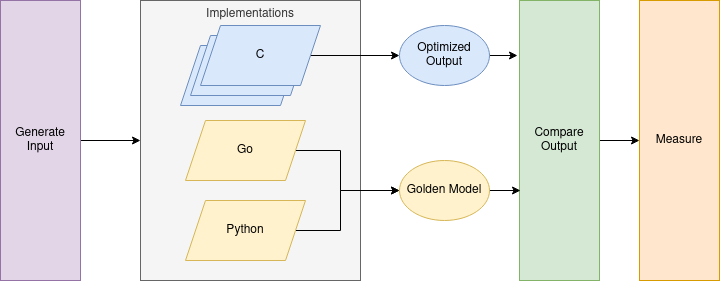
\includegraphics[width=0.4\textwidth]{img/setup.png}
    \caption{The Building, Testing and Benchmarking System}
    \label{img:setup}
\end{figure}

\mypar{Naive Implementation}
For APSP and MM, the naive implementation is as simple as possible, looking almost exactly like \ref{alg:fw}.
However, the naive implementation for TC already includes one optimization. The smallest datatype which C allows one to operate on is \texttt{char}. It has a size of 1 byte, or 8 bits.
But each of these bits is already enough to store a boolean value. The naive TC therefore already performs \emph{bit-packing}. That is a process wherein each byte accounts for 8 boolean values instead of just one.
This not only vastly reduces the space required to store and operate on matrices, but it also allows us to perform 8 logical operations at once, since taking the conjunction between two bytes actually performs eight bitwise conjunctions.

This is very similar to the later optimization of vectorization, as it essentially operates of vectors of 8 booleans each.

\mypar{Loop Unrolling}
Perhaps the most simple optimization performed in this project is \emph{loop unrolling}. Starting with the naive implementation, the two inner loops can be arbitrarily unrolled. But as mentioned earlier, the outermost loop cannot be unrolled, as it would violate dependencies.

In an additional, non-trivial optimization, the load of \texttt{C[i, k]} is moved out of the innermost loop. Furthermore, this value is not reloaded for the entire run of this loop.
At first, this optimization appears to be faulty, as the innermost loop can change \texttt{C[i, k]} if \texttt{j} is equal to \texttt{k}. However, in that case the update for APSP has the form of \texttt{C[i, k] = MIN(C[i, k], C[i, k] + C[k, k])}.
Since the algorithm requires the input graph not to have any negative circles, \texttt{C[k, k]} cannot be negative. Hence, \texttt{C[i, k] + C[k, k]} will never be smaller than just \texttt{C[i, k]}, meaning the update in question will never actually modify the value of \texttt{C[i, k]}.

For MM and TC, this optimization does not even require the input to fulfil any non-trivial problems. For MM, the update has the form \texttt{C[i, k] = MAX(C[i, k], MIN(C[i, k], C[k, k]))}, and for the TC it is \texttt{C[i, k] = C[i, k] | (C[i, k] \& C[k, k])}. In both cases, it is easy to see that the value of \texttt{C[i, k]} is left unchanged.

For easier understanding, a concrete example of unrolled code can be found in the appendix \ref{app:code}.

%At first, this implementation appears to be faulty: The value \texttt{cik = C[i, k]} is only read once for an entire run of the innermost loop. Yet, if the loop variable \texttt{j} is equal to \texttt{k}, the location \texttt{C[i, k]} can be overwritten. In such an event, it appears that \texttt{cik} would have to be read again, as its value might have changed. However, a closer examination of the problem at hand shows why this is not possible.
%The value that \texttt{C[i, k]} could be overwritten with, is computed as follows: \texttt{C[i, k] = MIN(C[i, k], C[i, k] + C[k, k])} (\emph{since we assume \texttt{k} and \texttt{j} are equal}). The only case in which this expression evaluates to something different from \texttt{C[i, k]} is if \texttt{C[k, k]} is negative. But since we explicitly require our graphs not to contain negative cycles, that is impossible.

\mypar{SIMD Vectorization}
\label{method:simd}
While certainly sounding more interesting, the introduction of SIMD (single instruction, multiple data) vector instructions is similar to just unrolling the innermost loop, but without all the additional load, compute and store statements. The unrolling factor depends on the data type the algorithm works with, as well as the hardware the program is to be run on.
For this project, we work with the \texttt{AVX} and \texttt{AVX2} vector instruction set, meaning the vector instructions work with vectors of 256 bits.
For the APSP and MM implementations, one such vector holds four doubles, meaning the innermost loops are essentially unrolled by a factor of four.
Regarding the TC, one such vector can hold 32 chars. This means that when compared to the naive implementation, the vectorized version unrolls the innermost loop by a factor of 32.

\mypar{Tiling}
This optimization is explained more thoroughly in section \ref{sec:background} and Alg. \ref{alg:fwt}. But in brief, the idea is to cut the matrix in tiles, and iterate over them. This not only allows for a faster loop ordering on some tiles, but if the tiles are of a suitable size, they also fit into the cache.
As a result, the processor has to spend significantly less time waiting for data, allowing it to more efficiently utilize its resources.

In addition to tiling, these implementations also have loop unrolling. In fact, using them with the tile size set to the entire input matrix is identical to using the unrolled version.

The tiled implementations are all parameterized by the tile size, which is set as high as possible such that three tiles fit into the machine's L2 cache.
To make the implementations more simple, we require the tile size divide the dimension of the input matrix, or the number of vertices in the input graph.
Furthermore, the tile size also has to be a multiple of the \emph{unrolling factor} of the functions operating on the tiles.

\mypar{Vectorized Tiling}
After the combination of tiling and unrolling, the obvious next step is to add vectorization too. As mentioned, vectorization is very similar to loop unrolling. The constraints on the tile size are therefore left unchanged for both the APSP and MM implementations.
However, in the case of TC, vectorization means that the unrolling factor becomes 256.
Coupled with the two constraints of dividing the input size and fitting into the cache, the vectorized tiled TC implementation is often forced to use significantly smaller tile sizes than would be optimal, leading to notable performance hits.
For a more stable implementation, the input matrix could be extended with zeros to allow for an optimal tile size. However, such an optimization is not part of this work.

\mypar{Autotuner}
In spite of the aforementioned constraints, there still is a vast number of possible parameters with which to implement a particular optimization, or a combination thereof.
Testing them all in order to find the best ones is therefore highly unpractical.
In addition, parameters that are optimal for one input size may not be the best for another size.
In order to find good parameters without tedious manual testing, we implement an autotuner, capable of testing parameters and searching good ones on its own.
While this autotuner is still unable perform an exhaustive search over all possible parameters, it can find locally optimal parameters and produce according code.

Figure \ref{img:autotuner} shows the process by which the autotuner formulates its guesses on suitable parameters, and then tries to refine them. It starts off by trying all possible parameters for an input size small enough to do so in reasonable time ($N=64$ in our case).
On the larger input size, the autotuner employs a hill-climbing algorithm to search for locally optimal parameters using the optimal parameter the algorithm found for a small input as an initial guess.
This algorithm again follows the illustrated process, where each round begins with the computation of parameter sets to try next. These parameter sets are generated by changing only one parameter of the current set, while leaving the rest unchanged. The new value for the changed parameter is always a neighbor of the current value, meaning either the next larger or next smaller value while respecting existing constraints.
In each round, the autotuner evaluates the performance on each of the generated parameter sets. If one of them surpasses the current best, the autotuner uses the according parameters as basis for the next round. And if it cannot find better parameters, it terminates, as a local optimum has been found.

Upon termination, the autotuner returns the locally optimal parameters it found, in addition to accordingly generated code. It works for each of the three semi-rings examined in this work. It can either perform unrolling, where it optimizes the unrolling factors, or it can perform both unrolling and tiling, where it optimizes the tile size and the unrolling factors. Furthermore, both versions support vectorization.

\begin{figure}[h]
    \centering
    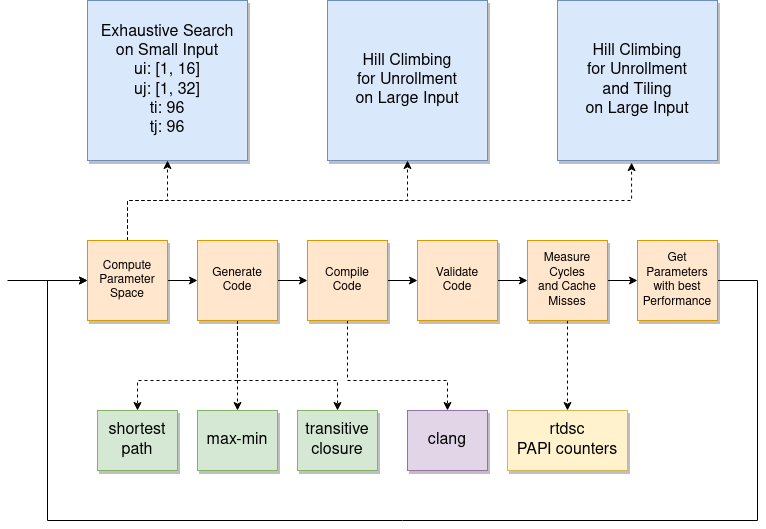
\includegraphics[width=0.4\textwidth]{img/autotuning.png}
    \caption{Autotuning Method}
    \label{img:autotuner}
\end{figure}

%Now comes the ``beef'' of the paper, where you explain what you
%did. Again, organize it in paragraphs with titles. As in every section
%you start with a very brief overview of the section.

%For this course, explain all the optimizations you performed. This mean, you first very briefly
%explain the baseline implementation, then go through locality and other optimizations, and finally SSE (every project will be slightly different of course). Show or mention relevant analysis or assumptions. A few examples: 1) Profiling may lead you to optimize one part first; 2) bandwidth plus data transfer analysis may show that it is memory bound; 3) it may be too hard to implement the algorithm in full generality: make assumptions and state them (e.g., we assume $n$ is divisible by 4; or, we consider only one type of input image); 4) explain how certain data accesses have poor locality. Generally, any type of analysis adds value to your work.

%As important as the final results is to show that you took a structured, organized approach to the optimization and that you explain why you did what you did.

%Mention and cite any external resources including library or other code.

%Good visuals or even brief code snippets to illustrate what you did are good. Pasting large amounts of code to fill the space is not good.
